\section{شبیه‌سازی استند سه درجه آزادی در محیط سیمولینک}\label{quadall3}
این بخش به بررسی و شبیه‌سازی مدل دینامیکی استند سه درجه آزادی پرداخته شده است. در بخش (\ref{spacestate}) فرم فضای حالت استند چهار پره استخراج شد. در شبیه‌سازی نیز از همین روابط استخراج شده استفاده شده است. مدل شبیه‌سازی شده از استند (شکل \ref{quadsimulink}) دارای چهار ورودی سرعت دورانی موتورها  و دارای سه خروجی زوایای رول ($\phi$)، پیچ ($\theta$)، یاو ($\psi$) و  سه سرعت‌های زاویه‌ای
 p
 q،
 و 
r 
 است.
 
 
\begin{figure}[H]
	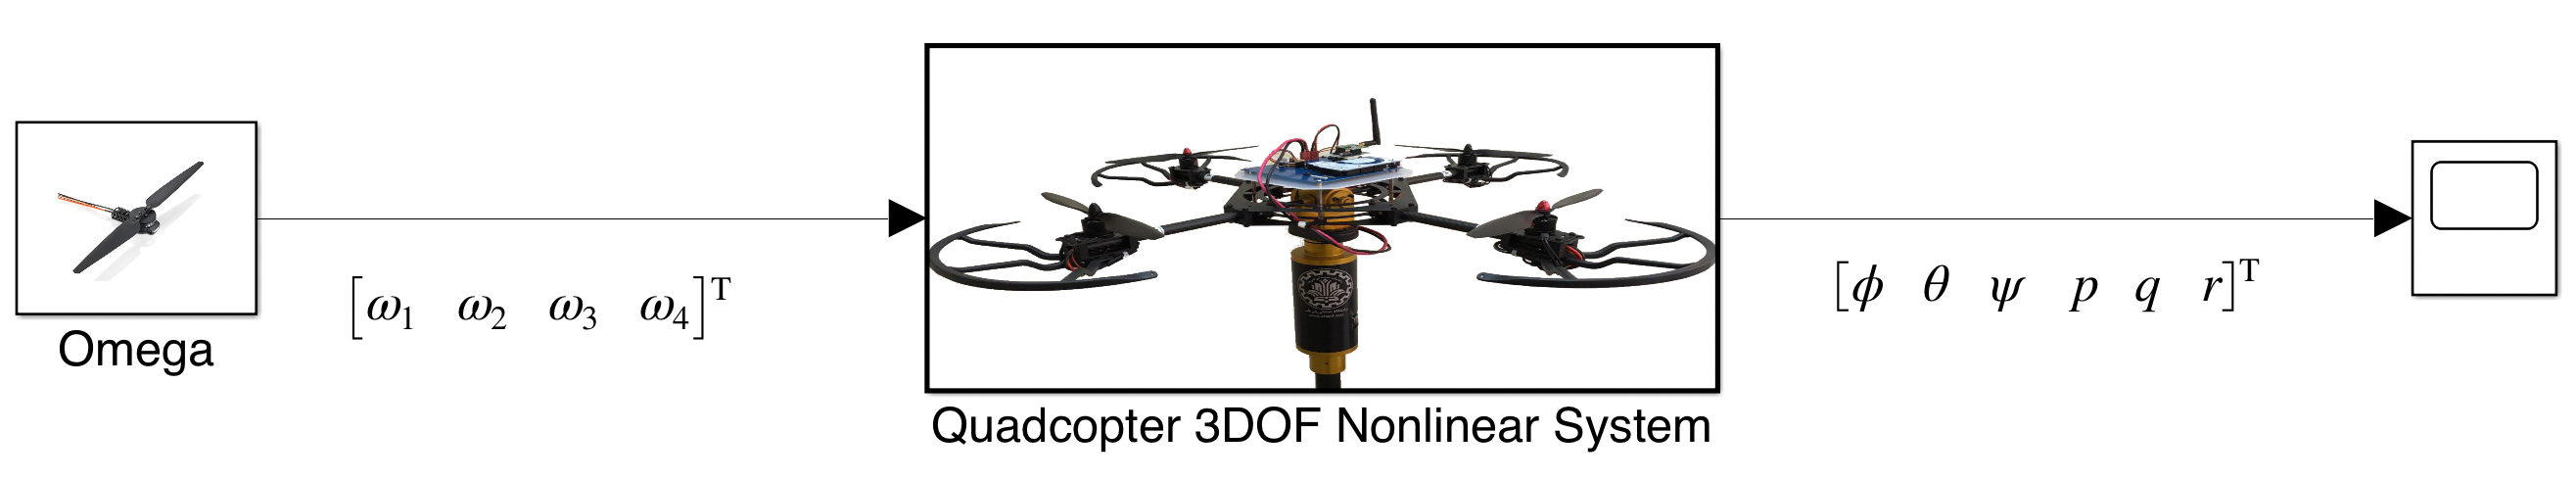
\includegraphics[width=16cm]{../../Figures/QuadSimulation/Stand_Model.png}
	\centering
	\vspace*{-15mm}
	\caption{مدل استند چهارپره شبیه‌سازی شده در سیمولینک و نمایش ورودی و خروجی‌های مدل}
	\label{quadsimulink}
\end{figure}
نمایی از داخل بلوک
\lr{Quacopter 3DOF Nonlinear System}
در شکل (\ref{Quad3DOF}) آورده شده است.
%\newline
%\newline
\begin{figure}[H]
	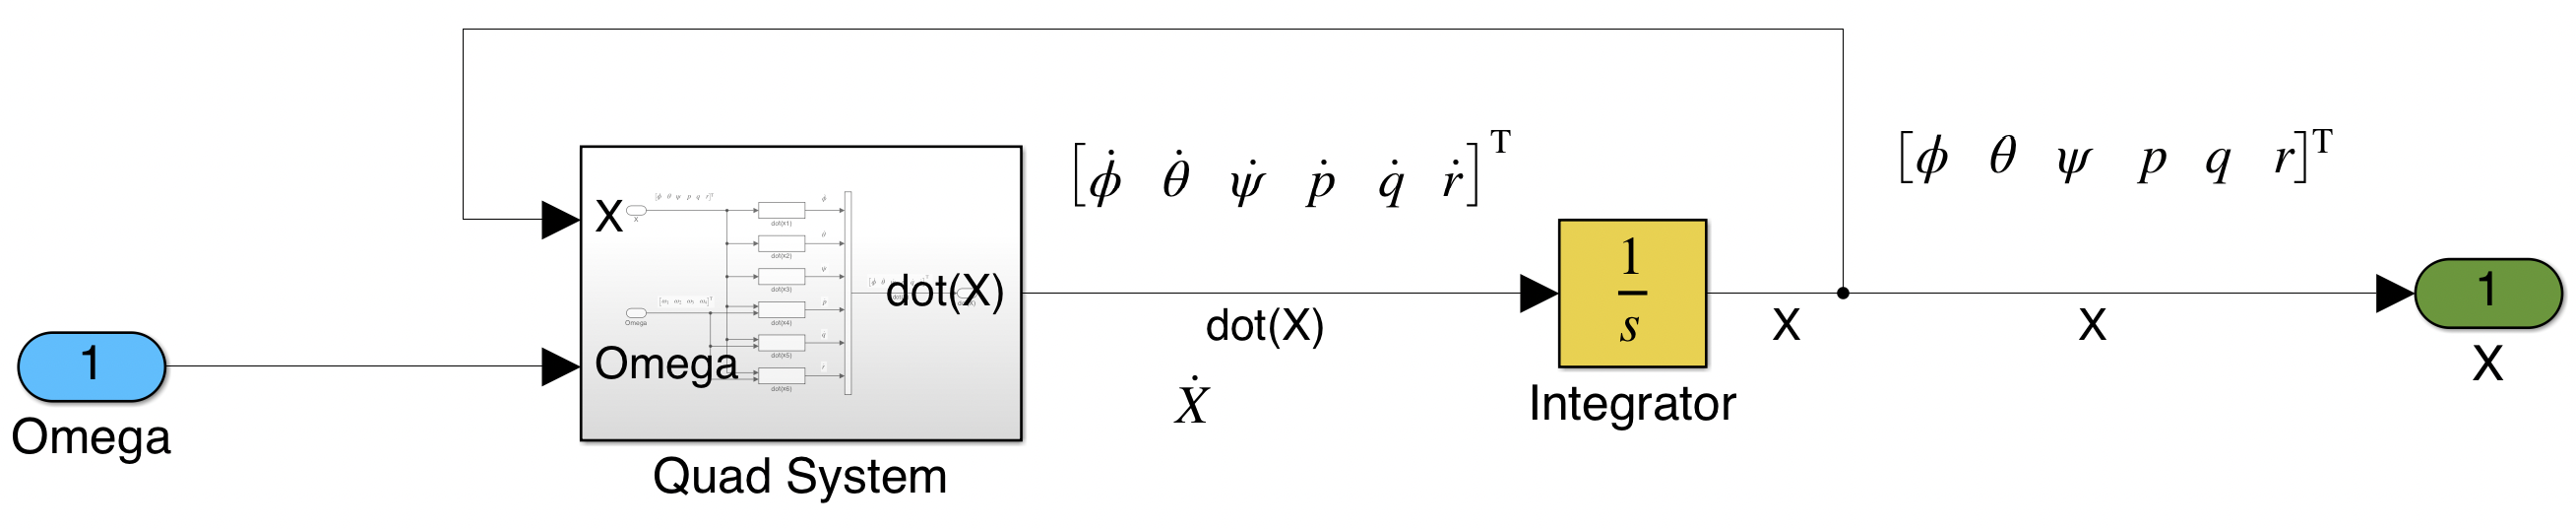
\includegraphics[width=16cm]{../../Figures/QuadSimulation/Integrator.png}
	\centering
	\vspace*{-15mm}
	\caption{مدل استند چهارپره شبیه‌سازی شده در سیمولینک و نمایش ورودی و خروجی‌های مدل}
	\label{Quad3DOF}
\end{figure}
بلوک
\lr{Quad System}،
$\dot X$ را به عنوان خروجی می‌دهد. با استفاده از بلوک انتگرالگیر (بلوک زرد رنگ) در شکل
(\ref{Quad3DOF})
از خروجی آن بر اساس شرایط اولیه استند انتگرال گرفته می‌شود و خروجی مورد نیاز ( زاویه‌های رول ($\phi$)، پیچ ($\theta$)، یاو ($\psi$) و سرعت‌های زاویه‌ای‌
p
q،
و 
r )
را می دهد.

داخل بلوک
\lr{Quad System}،
شش بلوک دارد که بعضی از آن‌های دارای ورودی $X$ و بعضی از آن‌های دارای ورودی $X$ و $\omega$ هستند. مجموع خروحی این شش بلوک $\dot X$ است که برای بلوک
\lr{Quad System}،
 نیز اشاره شد.
نمایی از داخل بلوک
\lr{Quad System}
در شکل (\ref{all-six}) آورده شده است.
\begin{figure}[H]
	\includegraphics[width=16cm]{../../Figures/QuadSimulation/all-six.png}
	\centering
%	\vspace*{-15mm}
	\caption{نمایی از داخل بلوک \lr{Quad System}}
	\label{all-six}
\end{figure}